\section{Анализ предметной области}
\label{sec:domain}

В данном разделе будет произведён обзор предметной области задачи, решаемой в рамках дипломного проекта.

\subsection{Теоретические основы}
\label{sub:domain:theory_basics}
Задача распознавания автомобильных номерных знаков относится к тами научным областям как теория распознавания образов и обработка изображений.
Обработка изображений — любая форма обработки информации, для которой входные данные представлены изображением, например, фотографиями или видеокадрами. Обработка изображений может осуществляться как для получения изображения на выходе (например, подготовка к полиграфическому тиражированию, к телетрансляции и т. д.), так и для получения другой информации (например, распознание текста, подсчёт числа и типа клеток в поле микроскопа и т. д.). Кроме статичных двухмерных изображений, обрабатывать требуется также изображения, изменяющиеся со временем, например, видео.~\cite{image_precessing}

Всю область можно охарактеризовать как молодую, разнообразную и динамично развивающуюся. Интенсивное её изучение началось лишь в конце 1970-х гг., когда компьютеры смогли управлять обработкой больших наборов данных, какими являются изображения. И сейчас нет стандартной формулировки этой области, а многие методы и приложения всё ещё находятся на стадии фундаментальных исследований. В последнее время наблюдается повышение активности изучения области, ввиду всё большего применения её методов в коммерческих продуктах.

Теория распознавания образа — раздел информатики и смежных дисциплин, развивающий основы и методы классификации и идентификации предметов, явлений, процессов, сигналов, ситуаций и т. п. объектов, которые характеризуются конечным набором некоторых свойств и признаков.
Для оптического распознавания образов можно применить метод перебора вида объекта под различными углами, масштабами, смещениями и т. д. Для букв нужно перебирать шрифт, свойства шрифта и т. д.
Второй подход — найти контур объекта и исследовать его свойства (связность, наличие углов и т. д.)
Ещё один подход — использовать искусственные нейронные сети. Этот метод требует либо большого количества примеров задачи распознавания (с правильными ответами), либо специальной структуры нейронной сети, учитывающей специфику конкретной задачи.

Обрабатывать мы будем растровые изображения. Растровое изображение — изображение, представляющее собой сетку пикселей — цветных точек.

В целом задача распознавания автомобильного номера сводится к следующим: 
\begin{itemize}
  \item обработка изображений;
  \item поиск номерного знака;
  \item поиск отдельных символов на рамке с номером;
  \item распознавание символа;
\end{itemize}

\subsection{Обработка изображений}
\label{sub:domain:image_processing}

Под обработкой  изображений понимают семейство  методов  и  задач,  где  входной  и  выходной информацией  являются  изображения~\cite{misoi_clides}. Обработка изображений обычно преследует одну из следующих целей:
\begin{itemize}
  \item улучшение качества изображения для восприятия человеком, т.е. сделать изображение лучше с субъективной точки зрения человека;
  \item улучшение изображение для восприятия компьютером, т.е. изменить изображение для упрощения последующего распознавания;
\end{itemize}
Типичные задачи для обработки изображений это корректировка яркости, цветов, освещения и устранение шумов. 

Многие алгоритмы распознавания изображение показывают хорошие результаты при правильной пред-обработке а некоторые и вовсе не работают без пред обработки. В заключение отмечу что алгоритмы пред-обработки выбираются исключительно из нужд алгоритмов распознавания.

Рассмотрим алгоритмы предобработки использующиеся в работе.

\subsubsection{}
\label{sub:domain:image_processing:edges_detection}
Выделение границ

Выделение границ (выделение краёв) — термин в теории обработки изображения и компьютерного зрения, частично из области поиска объектов и выделения объектов, основывается на алгоритмах, которые выделяют точки цифрового изображения, в которых резко изменяется яркость или есть другие виды неоднородностей.

Самым лучшим детектором границ считается детектор границ Кэнни~\cite{canny_edge_detector}. Потому как обладает следующими свойствами:
\begin{itemize}
  \item хорошее обнаружение (устойчивость к шуму);
  \item хорошая локализация (толщина выделенной границы получается 2 пикселя);
  \item единственный отклик на одну границу;
\end{itemize}

На рисунке \ref{fig:domain:image_processing:edges_detection:canny} виден пример работы детектора границ Кэнни. 

\begin{figure}[ht]
\centering
  \begin{subfigure}[b]{0.48\textwidth} 
    \centering
    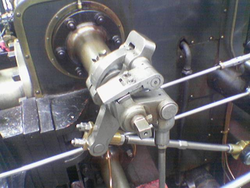
\includegraphics[width=\textwidth]{before_canny.PNG}  
    \caption{Исходное изображение}
  \end{subfigure}
  \begin{subfigure}[b]{0.48\textwidth} 
    \centering
    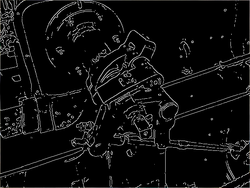
\includegraphics[width=\textwidth]{after_canny.PNG}  
    \caption{Обработанное изображение}
  \end{subfigure}
  \caption{Детектор границ Кэнни}
  \label{fig:domain:image_processing:edges_detection:canny}
\end{figure}


\subsubsection{}
\label{sub:temp:image_processing:binary}
Бинаризация

Бинаризация изображений - перевод полноцветного или в градациях серого изображения в монохромное, где присутствуют только два типа пикселей (темные и светлые)\cite{binary_image}. На рисунке \ref{fig:domain:image_processing:binary:binarization} виден пример бинаризации изображения.

\begin{figure}[ht]
\centering
  \begin{subfigure}[b]{0.48\textwidth} 
    \centering
    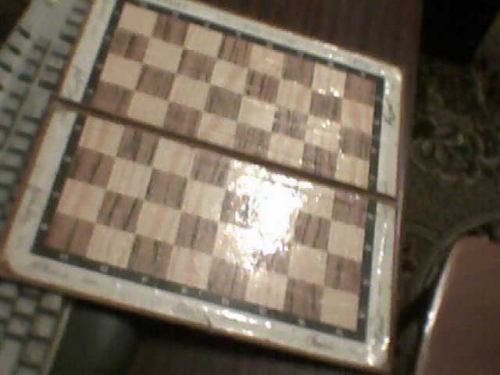
\includegraphics[width=\textwidth]{before_binarization.jpg}  
    \caption{Исходное изображение}
  \end{subfigure}
  \begin{subfigure}[b]{0.48\textwidth} 
    \centering
    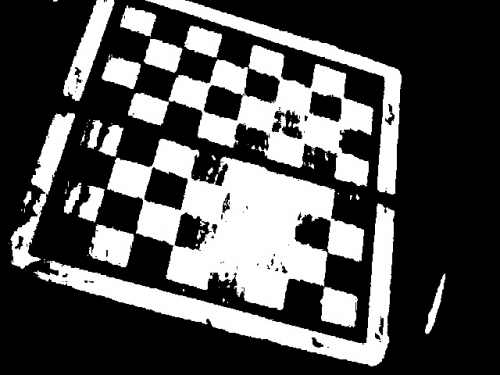
\includegraphics[width=\textwidth]{after_binarization.jpg}  
    \caption{Бинаризированое изображение}
  \end{subfigure}
  \caption{Бинаризация}
  \label{fig:domain:image_processing:binary:binarization}
\end{figure}

Алгоритм бинаризации несложен. Сперва требуется перевести изображение в оттенки серого использую формулу $ Y = 0.2126R + 0.7152G + 0.072B $, где Y значение градации серого, а R G и B значение каналов исходных цветов. Далее нужно сравнить значение каждого пикселя с неким пороговым значение и если значение превышает порог сделать пиксель темным и светлым если наоборот. 
Существуют различные подходы к выбору порогов, которые условно можно разделить на 2 группы:
\begin{itemize}
  \item Пороговые, которые ищут пороговое значение для изображение целиком
  \item Адаптивные, которые выбирают отдельный порог для каждого участка изображения, обычно используются при неравномерном освещении.
\end{itemize}


\subsection{Поиск номерного знака}
\label{sub:domain:search}
Рассмотрим возможные способы решения задачи поиска номерного знака.
\subsubsection{}
\label{sub:domain:search:edges_analisys}
Анализ границ и фигур.

Наиболее очевидный способ нахождение рамки это поиск прямоугольного контура. Для этого производится пред-обработка для поиска границ, например c помощью оператора Кэнни~\cite{canny_edge_detector}, затем ищутся все прямоугольники и анализируются на схожесть с государственным стандартом~\cite{stb_914_99} по соотношению сторон. Так же существует модификация~\cite{recognition_using_hought} при которой анализируется только часть рамки. Т.е. после выделения контуров ищутся вертикальные прямые и для любых прямых, расположенных недалеко друг от друга, с правильным соотношением расстояния между ними к их высоте, рассматривается гипотеза о том что номер располагается между ними. 


\begin{figure}[ht]
\centering
  \begin{subfigure}[b]{0.48\textwidth} 
    \centering
    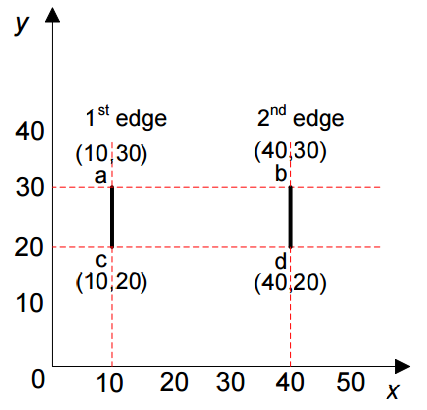
\includegraphics[width=\textwidth]{edge_analysis_graphic.png}  
    \caption{Координаты боковых границ номера}
  \end{subfigure}
  \begin{subfigure}[b]{0.48\textwidth} 
    \centering
    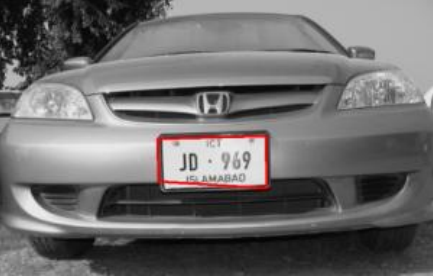
\includegraphics[width=\textwidth]{edge_analysis_recognized_plate.png}  
    \caption{Распознанная граница номера}
  \end{subfigure}
  \caption{Анализ границы номера}
  \label{fig:domain:search:edges_analisys:edge_graphic}
\end{figure}

В своей работе автор не указывает на каком компьютере он запускал описанный выше алгоритм, но заявленное время работы при обработке изображений 640 х 480 пикселей 0,3 секунды, что делает его практически пригодным для работы в режиме реального времени. На тесте из 102 изображений, алгоритм нашел номера на 96 из них.

\subsubsection{}
\label{sub:domain:search:histogram_analisys}
Анализ гистограмм.

Гистограмма - это график статистического распределения элементов цифрового изображения с различной яркостью, в котором по горизонтальной оси представлена яркость, а по вертикали — относительное число пикселов с конкретным значением яркости.~\cite{color_histogram}

\begin{figure}[ht]
\centering
    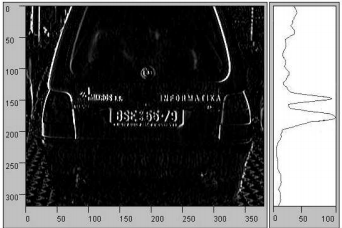
\includegraphics[scale=0.8]{histogram_after_edge_detection.png}  
    \caption{Вертикальная гистограмма после фильтра границ}
    \label{fig:domain:search:edges_analisys:vertical_histogram_after_edge_detection}
\end{figure}

Анализ гистограмм обрел большую популярность так как встречается сразу в нескольких работах ~\cite{recognition_using_histogram_1}~\cite{recognition_using_histogram_2}. 
Идея заключается в пред-обработке изображение фильтром границ с построением гистограммы в последующем. На рисунке \ref{fig:domain:search:edges_analisys:vertical_histogram_after_edge_detection} отчетливо виден всплеск на гистограмме в области автомобильного номера. Анализирую изменения на вертикальной и горизонтальной гистограмме можно вычислить положение автомобильного номера. 

Рассмотренный метод имеет достаточную производительность чтобы работать в режиме реального времени: при использовании компьютера с центральным процессором работающем на частоте 3.0 GHz и имеющем 512 MB оперативной памяти справлялся с обработкой изображения 320 на 240 пикселя в среднем 0.07 секунд.

Главным недостатком анализа гистограмм является существенное ограничение на входные данные: машина должны занимать значительную площадь на изображении и туда не должно попадать постороннего текста, который легко может стать причиной лишних всплесков на гистограмме.

\subsubsection{}
\label{sub:domain:search:violajones}
Метод Виолы - Джонса.

Метод Виолы - Джонса  это первый алгоритм обнаружения объектов работающий в режиме реального времени предложенный Paul Viola и Michael Jones в 2001 году~\cite{viola_jones_wiki}~\cite{viola_jones_habr}. Алгоритм использует компьютерное обучение с учителем и может быть обучен для распознавания различных объектов, во время разработки метода перед авторами стояла задача распознавание лица. 

Метод основан на следующих принципах:
\begin{itemize}
  \item используются изображения в интегральном представлении, что позволяет вычислять быстро необходимые объекты;
  \item используются признаки Хаара, с помощью которых происходит поиск нужного объекта;
  \item используется бустинг для выбора наиболее подходящих признаков для искомого объекта на данной части изображения;
  \item все признаки поступают на вход классификатора, который даёт результат «верно» либо «ложь»;
  \item используются каскады признаков для быстрого отбрасывания окон, где не найдено лицо.
\end{itemize}

Для работы с изображением оно переводится в интегральное представление. Интегральное представление изображения это матрица, равная по размерам исходному изображению, в каждом элементе которой хранится сумма интенсивностей все пикселей находящихся левее выше данного элемента. Другими словами каждый элемент матрицы интегрального представления можно расчитать по формуле 
$ L_{x,y} = \sum_{i=0,j=0}^{i \leq x, j \leq y} I_{i,j} $, где $L_{x,y}$ это элемент матрицы интегрального представления с координатами $xy$, а $I_{i,j}$ это интенсивность пикселя исходного изображения с координатами $ij$.
При дальнейшем рассмотрении алгоритма мы убедимся что такое представление данных может сократить время вычислений.

Основа метода виолы джонса это признаки Хаара. Признаки Хаара это признак цифрового изображения вычисляемый на основе примитива Хаара. В методе Волы - Джонса используются прямоугольные примитивы Хаара представленные на рисунке \ref{fig:domain:search:violajones:haar_features}. Вычисляемым значением признака будет $F = A - B$, где $A$ - сумма интенсивностей закрываемой светлой частью признака, а $B$ - сумма яркостей закрываемая темной частью признака. Для вычисления признаков Хаара очень удобно использовать интегральное представление изображения описанное ранее, т.к. оно позволяет вычислять разницу интенсивности областей изображения не за линейное время $o(n)$ а за постоянное $o(1)$. По отдельности признаки Хаара являются слабым классификатором с большой вероятностью ошибки, но работающие очень быстро. 

\begin{figure}[ht]
\centering
  \begin{subfigure}[b]{0.4\textwidth} 
    \centering
    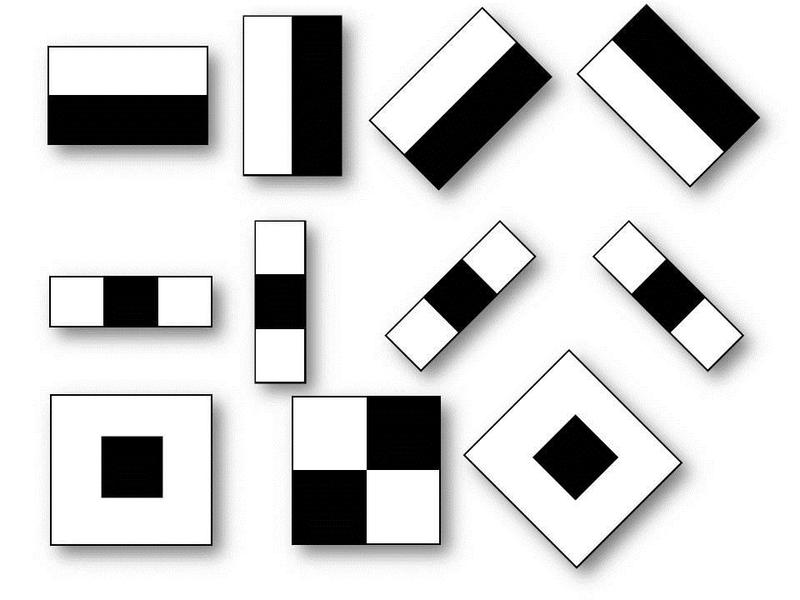
\includegraphics[width=\textwidth]{haar_features.jpg}  
    \caption{Оригинальные примитивы}
  \end{subfigure}
  \begin{subfigure}[b]{0.4\textwidth} 
    \centering
    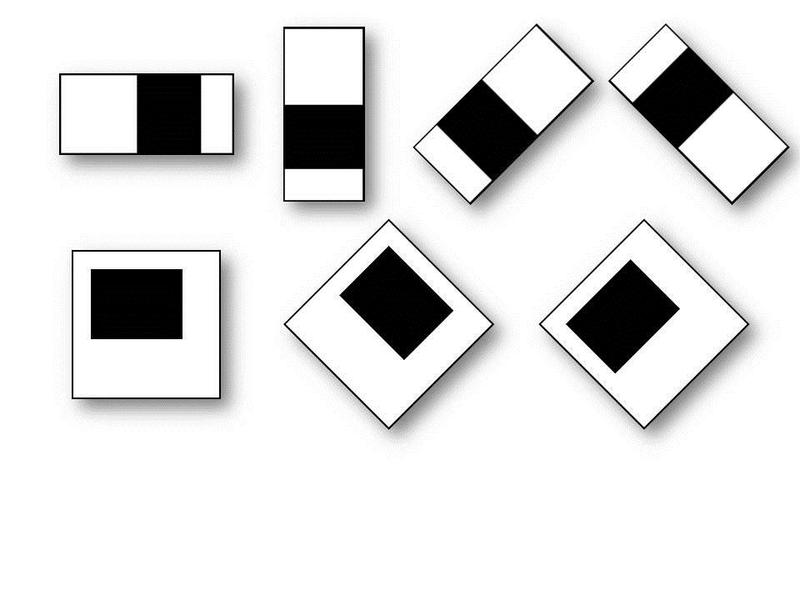
\includegraphics[width=\textwidth]{haar_features_additional.jpg}  
    \caption{Дополнительные примитивы}
  \end{subfigure}
  \caption{Примитивы Хаара}
  \label{fig:domain:search:violajones:haar_features}
\end{figure}

Непосредственно обработка изображение в методе Виолы - Джонса осуществляется сканирующим окном. Работает это следующим образом: изображение разбивается на ячейки и сканирующее окно начинает идти по ячейкам высчитывая требуемые признаки Хара для ячейки, при этом сканирование происходит последовательно при различных масштабах, но масштабируется не само изображения а сканирующее окно. Обращу внимание на то что обработка таким образом легко распараллеливается что очень хорошо сказывается на скорости выполнения, так как большинство машин на сегодняшний день именно многоядерные. 

Обучение алгоритма происходит с помощью компьютерного обучения с учителем, т.е. алгоритму нужна конечная обучающая выборка классифицированных объектов, для которых будут расчитаны и сохраненны каскады Хаара. Обучение занимает очень много времени: от дней до нескольких недель.

Вообще классификаторы можно разделить на 2 типа: слабые и сильные. Эффективный классификатор допускающий мало ошибок называют сильным, классификатор допускающий много ошибок называют слабым. Но слабые классификаторы работают значительно, значительно быстрее сильных. Метод Виолы - Джонса как уже было рассмотренно основан на слабых классификаторах - признаках Хаара, они работают очень быстро а точность достигается за счет бустинга. Бустинг - процедура последовательного построения композиции алгоритмов машинного обучения, когда каждый следующий алгоритм стремится компенсировать недостатки предыдущего. 

Идея бустинга была предложена Йоавом Фреундом и Робертом Шапиром в конце 90-х годов \cite{boosting}, когда надо было найти решение вопроса о том, чтобы имея множество плохих (незначительно отличающихся от случайных) алгоритмов обучения, получить один хороший. В основе такой идеи лежит построение цепочки (ансамбля) классификаторов, который называется каскадом, каждый из которых (кроме первого) обучается на ошибках предыдущего. 
Например, один из первых алгоритмов бустинга Boost1 использовал каскад из 3-х моделей, первая из которых обучалась на всем наборе данных, вторая – на выборке примеров, в половине из которых первая дала правильные ответы, а третья — на примерах, где ответы первых двух разошлись. Таким образом, имеет место последовательная обработка примеров каскадом классификаторов, причем так, что задача для каждого последующего становится труднее. Результат определяется путем простого голосования: пример относится к тому классу, который выдан большинством моделей каскада.

Развитием данного подхода явилась разработка более совершенного семейства алгоритмов бустинга AdaBoost, с английского adaptive boosting это адаптированное улучшение, который может использовать произвольное число классификаторов и производить обучение на одном наборе примеров, поочередно применяя их на различных шагах.

Подводя итог вышесказанного можно отметить что метод Виолы - Джонса основан на построении каскада слабых классификаторов алгоритмом AdaBoost применяемых при сканировании изображения скользящим окном.

Главным преимуществом метода Виолы - Джонса перед рассмотренными ранее алгоритмами является обучаемость. Во время выполнения работы мы можем собирать изображения автомобилей и добавлять их в обучающую выборку тем самым улучшая качество распознавания не меняя алгоритма, так же при появлении нераспознаваемого случая его можно просто включить в обучающую выборку и переобучить алгоритм. Я считаю что именно метод Виолы - Джонса лучше всего подходит для задачи нахождения автомобильного номера для последующего распознавания.

\subsection{Распознавание текста}
\label{sub:domain:recognition}

После выделения номерного знака на изображении можно приступить к распознаванию текста на табличке. 
Имеется ряд существенных проблем, связанных с распознаванием рукописных и печатных символов. Наиболее важные из них следующие:
\begin{itemize}
  \item разнообразие форм начертания символов;
  \item искажение изображений символов;
  \item вариации размеров и масштаба символов.
\end{itemize}
К счастью номерные знаки имеют стандарты по шрифтам и написанию, поэтому проблема с разнообразием форм автоматически отпадает.

Вобщем для распознавания текста требуется проделать следующие шаги
\begin{itemize}
  \item локализировать и выделать элементы текста;
  \item пред-обработать изображение;
  \item выделить признаки
  \item распознать символы
\end{itemize}

Для локализации и обработки используются следующие алгоритмы сегментации либо выделения границ. После этих операций можно произвести анализ и выделить текст. Имея точное положение рамки задача становится не сложной.

Считается, что выделение признаков является одной из наиболее трудных и важных задач в распознавании образов. Для распознавания символов может быть использовано большое количество различных систем признаков. Проблема заключается в том, чтобы выделить именно те признаки, которые позволят эффективно отличать один класс символов от всех остальных в данной конкретной задаче.
Ниже описан ряд основных методов распознавания символов и соответствующих им типов признаков, вычисляемых на основе цифрового изображения.

\subsubsection{}
\label{sub:domain:recognition:compare_with_template}
Сопоставление изображений и шаблонов

Эта группа методов основана на непосредственном сравнении изображений тестового и эталонного символов. При этом вычисляется степень сходства между образом и каждым из эталонов. Классификация тестируемого изображения символа происходит по методу ближайшего соседа. 

С практической точки зрения эти методы легко реализовать, и многие коммерческие системы OCR используют именно их. Однако при "лобовой" реализации корреляционных методов даже небольшое темное пятнышко, попавшее на внешний контур символа, может существенно повлиять на результат распознавания. Так же как недостаток можно отметить

\subsubsection{}
\label{sub:domain:recognition:statistic_analisys}
Статистические характеристики.

В данной группе методов выделение признаков осуществляется на основе анализа различных по статистических распределений точек. Наиболее известные методики этой группы используют вычисление моментов и подсчет пересечений.

Моменты различных порядков с успехом используются в самых различных областях машинного зрения в качестве дескрипторов формы выделенных областей и объектов. В случае распознавания текстовых символов в качестве набора признаков используют значения моментов совокупности "черных" точек относительно некоторого выбранного центра. Наиболее общеупотребительными в приложениях такого рода являются построчные, центральные и нормированные моменты.
Для цифрового изображения, хранящегося в двумерном массиве, построчные моменты являются функциями координат каждой точки изображения следующего вида: $$ m_{pq} =\sum\limits_{x=0}^{M-1} {\sum\limits_{y=0}^{N-1} {x^py^qf(x,y)} } , $$ где $p,q \in \{0,1,\ldots ,\infty \}$; $M$ и $N$ являются размерами изображения по горизонтали и вертикали и $f(x,y)$ является яркостью пиксела в точке $\langle x,y\rangle$ на изображении.
Центральные моменты являются функцией расстояния точки от центра тяжести символа: $$ m_{pq} =\sum\limits_{x=0}^{M-1} {\sum\limits_{y=0}^{N-1} {(x-\mathop x\limits^\_ )^p(y-\mathop y\limits^\_ )^qf(x,y)} } , $$ где $x$ и $y$ "с чертой" - координаты центра тяжести.
Нормированные центральные моменты получаются в результате деления центральных моментов на моменты нулевого порядка.
Следует отметить, что строковые моменты, как правило, обеспечивают более низкий уровень распознавания. Центральные и нормированные моменты более предпочтительны вследствие их большей инвариантности к преобразованиям изображений.

В методе пересечений признаки формируются путем подсчета того, сколько раз и каким образом произошло пересечение изображения символа с выбранными прямыми, проводимыми под определенными углами. Этот метод часто используется в коммерческих системах благодаря тому, что он инвариантен к дисторсии и небольшим стилистическим вариациям написания символов, а также обладает достаточно высокой скоростью и не требует высоких вычислительных затрат. На рисунке \ref{fig:domain:recognition:statistic_analisys:crossing_list} показано изображение символа R, и система секущих прямых.

\begin{figure}[ht]
\centering
  \begin{subfigure}[b]{0.4\textwidth} 
    \centering
    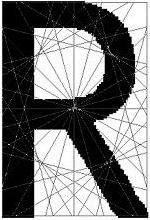
\includegraphics[scale=0.7]{crossing-example.jpg}  
    \caption{Эталонное изображение}
  \end{subfigure}
  \begin{subfigure}[b]{0.4\textwidth} 
    \centering
    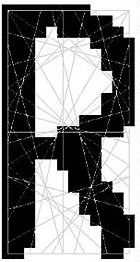
\includegraphics[scale=0.6]{crossing-for-real.jpg}  
    \caption{Реальное изображение}
  \end{subfigure}
  \caption{Пример формирования набора пересечений}
  \label{fig:domain:recognition:statistic_analisys:crossing_list}
\end{figure}

Метод зон предполагает разделение площади рамки, объемлющий символ, на области и последующее использование плотностей точек в различных областях в качестве набора характерных признаков. На \ref{fig:domain:recognition:statistic_analisys:zones_description} показано изображение символа R. На обоих изображениях приводятся разбиение на зоны, пиксельные веса каждой зоны, а также вектор расстояний до эталонных векторов эталонных символов.

\begin{figure}[ht]
\centering
  \begin{subfigure}[b]{0.4\textwidth} 
    \centering
    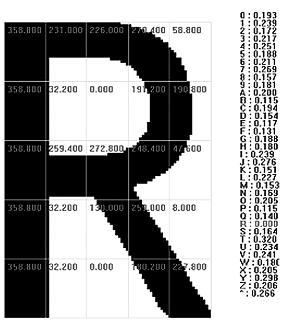
\includegraphics[scale=0.5]{zone-methods-example.jpg}  
    \caption{Эталонное изображение}
  \end{subfigure}
  \begin{subfigure}[b]{0.4\textwidth} 
    \centering
    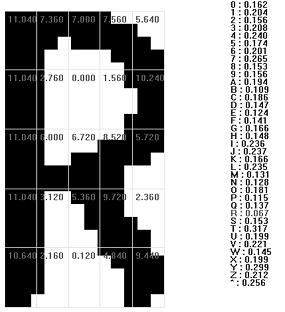
\includegraphics[scale=0.4]{zone-method-real.jpg}  
    \caption{Реальное изображение}
  \end{subfigure}
  \caption{Пример формирования зонного описания}
  \label{fig:domain:recognition:statistic_analisys:zones_description}
\end{figure}

В методе матриц смежности в качестве признаков рассматриваются частоты совместной встречаемости "черных" и "белых" элементов в различных геометрических комбинациях. Метод характеристических мест использует в качестве признака число раз, которое вертикальный и горизонтальный векторы пересекают отрезки линий для каждой светлой точки в области фона символа.


\subsubsection{}
\label{sub:domain:recognition:integral_transformation}
Интегральные преобразование

Среди современных технологий распознавания, основанных на преобразованиях, выделяются методы, использующие Фурье-дескрипторы символов, а также частотные дескрипторы границ.
Преимущества методов, использующих преобразования Фурье - Меллина, связаны с тем, что они обладают инвариантностью к масштабированию, вращению и сдвигу символа. Основной недостаток этих методов заключается в нечувствительности к резким скачкам яркости на границах, к примеру, по спектру пространственных частот сложно отличить символ "O" от символа "Q" и т. п. В то же время, при фильтрации шума на границах символа, это свойство может оказаться полезным.

\subsubsection{}
\label{sub:domain:recognition:contour_anolisys}
Анализ связанности контуров

На текущим момент большую популярность обрел способ при котором анализируется связанность контуров. Это дает множество преимуществ по сравнению с остальными методами: например это единственны метода который позволяет распозновать как черный текст на белом фоне так и белый текст на черном фоне. Анализ контуров это сложная задача и её решают при помощи самообучающихся классификаторов.  


\subsection{Обзор аналогов}
\label{sub:domain:analogs}

\subsubsection{}
\label{sub:domain:realization:automarshal}
Автомаршал 

Автомаршал – программное обеспечение для распознавания номеров автомобилей. Применяется для автоматизации парковок, весовых, КПП, автомоек, ТСЖ и т.п.\cite{auto_marshal}
Достоинства:
\begin{itemize}
  \item имеются версии распознающие номера на скорости до 150 км/ч;
  \item поддерживаются номерные знаки большого количества стран: Российская Федерация, Казахстан, Украина, Белоруссия, Киргизия, Узбекистан, Нидерланды, Польша, Бельгия, Германия;
\end{itemize}
Недостатки:
\begin{itemize}
  \item интегрируется только с *.xls, *.xlsx, *.csv базами данных, т.е не подходит для компаний с развитой IT инфраструктурой;
  \item высокая цена, которая зависи от количества камер и стран, чьи регистрационные знаки распознаются;
  \item работает только на \windows{} серверах;
  \item нет возможности попробовать перед покупкой;
\end{itemize}

\subsubsection{}
\label{sub:domain:analogs:alpha_systems}
Альфа системз

Модуль распознавания автомобильных номеров - Альфа системз~\cite{alpha_system}. Модуль распознавания автомобильных номеров автоматически определяет и распознает номера автомобилей в поле зрения камеры. Он позволяет фиксировать и сохранять в базе данных SQL распознанный номер, а также изображение транспортного средства, часть кадра с номерным знаком и время регистрации. Таким образом, формируется база всех транспортных средств, прошедших через зону контроля, с возможностью добавления текстового комментария к каждому распознанному номеру. В совокупности с модулем «Радар», предоставляющем информацию о скорости автомобилей, модуль распознавания автомобильных номеров может использоваться ГИБДД для регистрации нарушителей скоростного режима. Есть возможность сравнения распознаваемых номеров со сторонней базой номеров (например, автомобилей, числящихся в угоне), что позволяет применять модуль для целей розыска. Другим важным применением модуля является его использование в системах автоматического учета и контроля доступа автотранспорта на охраняемые объекты и платные автостоянки.
Достоинства:
\begin{itemize}
  \item работает с SQL базами данных;
  \item поддерживаются номерные знаки большого количества стран: Российской Федерации, Беларуси, Украины, Молдавии, Казахстана, Узбекистана, Латвии, Эстонии, Польши, Германии, Испании, Бразилии, Кубы;
\end{itemize}
Недостатки:
\begin{itemize}
  \item возможность интеграции лучше чем у Автомаршала(\ref{sub:domain:realization:automarshal}) но все ещё не достаточно хороша: нет точки расширения для интегрирования с имеющимися rest сервисами компании;
  \item высокая и непрозрачная цена;
  \item работает только на \windows{} серверах;
  \item нет возможности попробовать перед покупкой;
\end{itemize}

\subsubsection{}
Autonomerok

Распознаватель авто номеров - autonomerok. Autonomerok - производит распознавание номера машины в потоке, сохранение события с записью номера, времени и кадра с номером, а также может управлять исполнительными устройствами. Программа будет отлично работать c аналоговыми IP видеокамерами разных производителей.
\begin{itemize}
  \item работает с SQL light базой данных;
  \item есть возможность проверить перед покупкой;
\end{itemize}
Недостатки:
\begin{itemize}
  \item возможность интеграции лучше чем у Автомаршала(\ref{sub:domain:realization:automarshal}) но все ещё не достаточно хороша: нет точки расширения для интегрирования с имеющимися rest сервисами компании;
  \item высокая цена;
  \item работает только на \windows{} серверах;
  \item небольшая количество по сравнению с Автомаршалом(\ref{sub:domain:realization:automarshal}) и Альфи системз(\ref{sub:domain:analogs:alpha_systems}), количество поддерживаемых типов номерных знаков.
\end{itemize}

\subsubsection{}
Резюме обзора аналогов

Все имеющиеся приложения имеют высокую цену и лишний для нашей задачи функционал. Они позиционирую себя как готовые решения для платных парковок, авто моек и т.п. и расчитаны больше на малые компании и частных предпринимателей, у которых нет развитой информационной инфраструктуры. 

\subsection{Постановка целей и задач дипломного проекта}
Цель - разработка программного средства для автоматизации автомобильной стоянки компании \company{}.


Задачи:
\begin{itemize}
  \item Разработка архитектуры ПС;
  \item Разработка алгоритмов;
  \item Выбор платформы для разработки программного средства;
  \item Разработка пользовательского интерфейса;
  \item Создание базового проекта в среде программирования;
  \item Создание пользовательского интерфейса;
  \item Программирование и тестирование модулей;
  \item Сборка и тестирование ПС;
\end{itemize}
